\Chapter{Related Work}\label{chapter:related}

% What is data, information, knowledge?

The earliest work discussing information and similar concepts comes from Shannon in 1948\cite{shannon1948mathematical}.
The author however never defines the term itself and simply proposes models for quantitative analysis.
Approach described back then was more related to data than it was to information.
The distinction was made clear by Langefors in 1973\cite{langefors1973theoretical}.
Langefors proposed an approach putting the users of information first and proposed the following equation to describe the interaction of time, data, knowledge and information:
$$
    I = i(D, S,t)
$$
where:
\begin{variables}
    $I$ & information \\
    $i$ & interpretation process \\
    $D$ & data \\
    $S$ & knowledge \\
    $t$ & time
\end{variables}
In 1989, Ackoff\cite{ackoff1989data} defined the hierarchy of the human mind as consisting of wisdom at the very top and descending into understanding, knowledge, information and further into data.
The more popularized variant of this hierarchy being DIKW (data, information, knowledge, wisdom), became widespread in literature regarding knowledge management\cite{skyrme2007knowledge}.
There have been many attempts to define the distinction between these terms as well as the terms themselves.
One notable example was done by Grabowski and Zając in 2009\cite{mariusz2009dane}.
\begin{figure}[h]
    \centering
    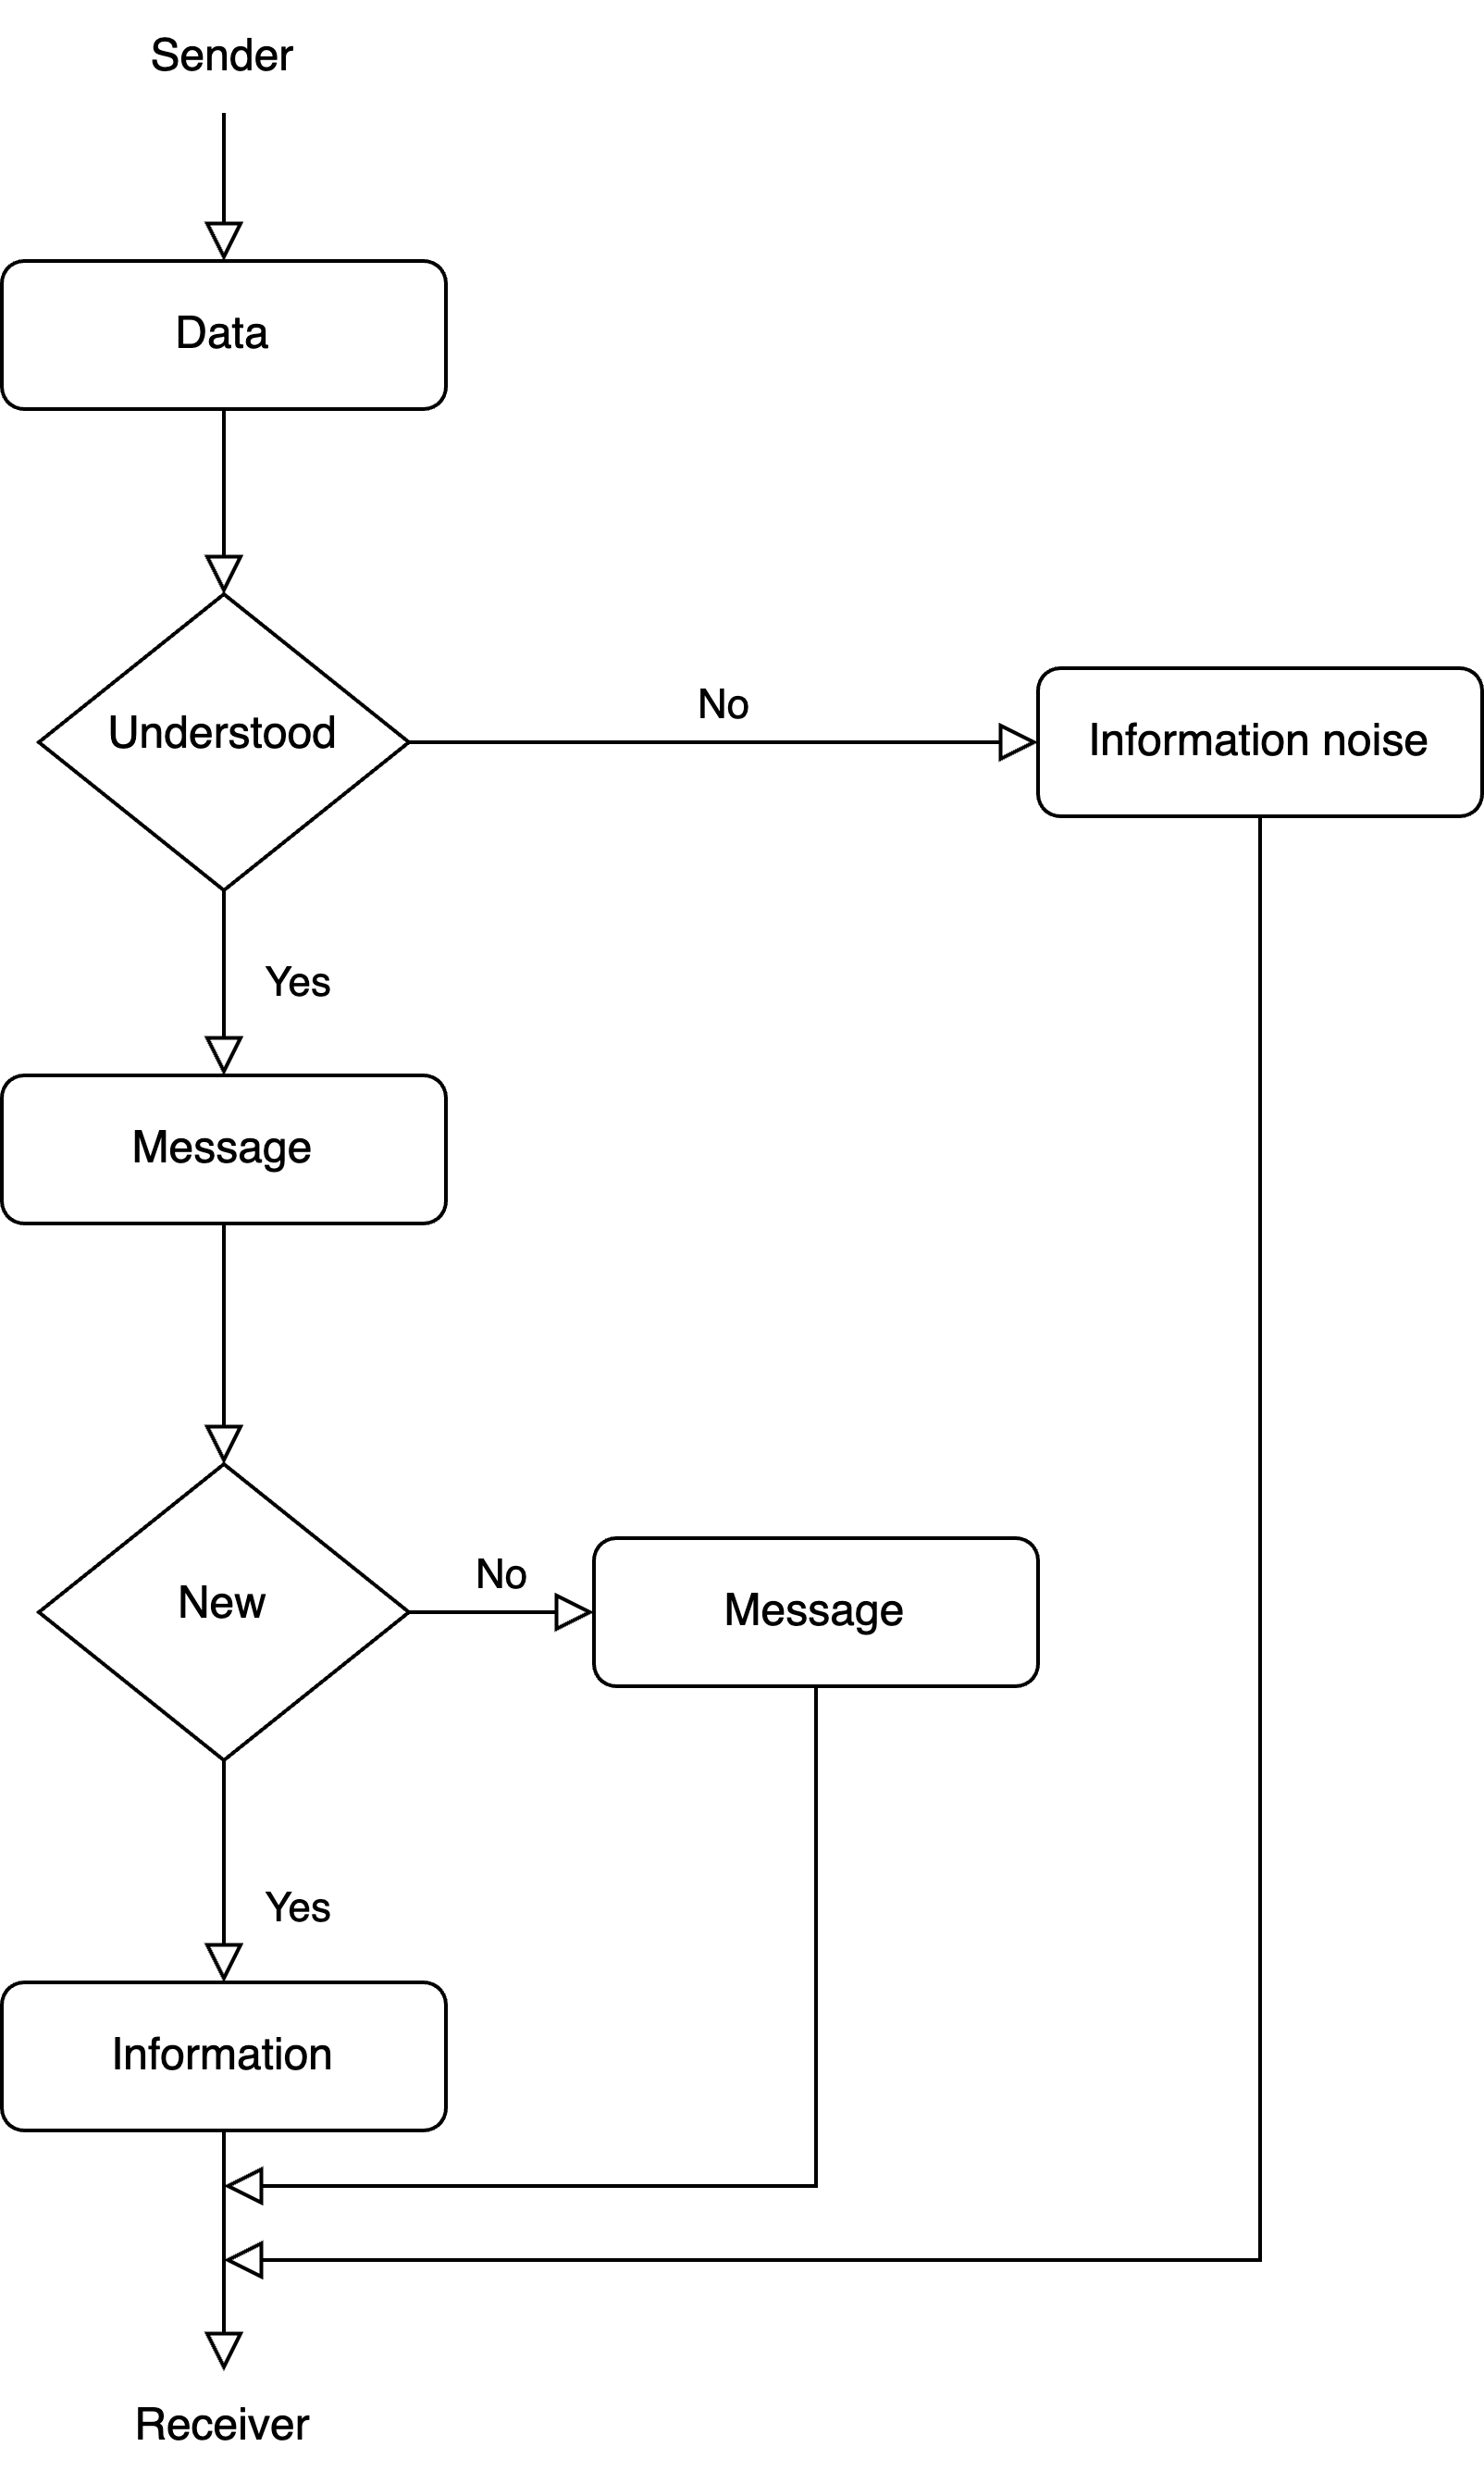
\includegraphics[width=0.6\textwidth]{images/od_nadawcy_do_odbiorcy.png}
    \caption{Information flow\cite{mariusz2009dane}}\label{fig:od_nadawcy_do_odbiorcy}
\end{figure}
The authors stress the hardship of definition of such primal terms and highlight the two major science disciplines that are related to them (information theory and knowledge management).
Both disciplines use the pyramid of knowledge (or information respectively).
According to Liew\cite{liew2013dikiw} trying to accurately define data, information and knowledge will result in circular definition.
To solve that problem he proposes a DIKIW model where "I" stands for "Intelligence".
Irrespective of chosen framework, everyone agrees that information and knowledge are related but represent different levels of abstraction.
While data is raw and unprocessed before it can become information, similarly information needs to be retained and assimilated to become knowledge.
The scope of this thesis covers only information understood as statements of fact and knowledge defined as retained and processed information.

A population of people can be said to possess knowledge similarly to a single individual.
Often a crowd has greater knowledge than any individual.
Surowiecki said "under the right circumstances, groups are remarkably intelligent, and are often smarter than the smartest people among them"\cite{surowiecki2005wisdom}.
To understand how knowledge is gained within a population one should analyze the way information itself is propagated.
In fact, people have already noticed that certain facts, stories or news share similarities with viral infections in how they spread across the whole population and eventually die out.
One such example is the work done by Liu et al.\cite{liu2016} where the authors describe how information spread can be explained using epidemiological models.
Truly, the simplest of such models called SIR\cite{weiss2013sir} can be used to describe in simple terms how a population can be partitioned into groups of \emph{Susceptible} (people who haven't encountered the viral information yet), \emph{Infected} (those who know the news and are willing to share it) and \emph{Removed} (everyone who either lost interest or simply never exhibited it).
There are however differences between infectious diseases and information.
For this reason variations of the SIR model became born.
Zhao et al.\cite{zhao2012sihr} have developed the SIHR model where H stands for \emph{Hibernators}.
The authors stress the importance of forgetting and remembering in trying to model the spread of information.
Another variation worth noting is the SCIR model consisting of \emph{Susceptible}, \emph{Contacted}, \emph{Infected} and \emph{Refractory}\cite{xiong2012scir}.
Both models use complex systems in order to simulate information propagation.
Other attempts at modelling information propagation are networks\cite{rodriguez2013} and cellular automata\cite{silva2020}.
Most literature dealing with the topic refers to social media, blogs and internet as the main medium of information exchange.
Relatively few works analyze the mechanisms behind word-of-mouth communication.
In 2003 at the "Symposium on Applications and the Internet", Takeuchi, S. and Kamahara, J. and Shimojo, S. and Miyahara, H. have presented their work titled "Human-network-based filtering: the information propagation model based on word-of-mouth communication" which deals with simulating how certain information is spread based on the filters of interest\cite{takeuchi1183031}.
Most authors treat knowledge of information as a binary value.
In reality the level of knowledge is often more complicated.
Silva et al.\cite{silva2020} propose the application of cellular automata to model information expressed as a linear value.

When trying to model how information propagates in a given system, it is often helpful to try and list its characteristics.
Grabowski and Zając followed the steps of Langefors and others while describing the following set of information characteristics:
\begin{itemize}
    \item Completedness - information must inlude context necessary for its interpretation
    \item Versatility - information should be interpretable from multiple viewpoints
    \item Accuracy - it should not be too vague nor too specific
    \item Financially viable - it should be useful in business context
\end{itemize}
These show clearly how most work done previously in this domain of knowledge related to the business context.
The domain of information propagation modelling seems to lack any work done in the context of game development.